\documentclass{mywork}
\blattnla

\begin{document}
	\begin{aufgabe}~

		Stelle jeweils das Gleichungssystem mit der Vandermonde-Matrix auf und löse.
		\begin{enumerate}[a)]
			\item
				Funktionsgleichung:
				\[
					ax^2 + bx + c
				\]
				Löse das Gleichungssystem
				\[
					\begin{pmatrix}1&-1&1\\1&0&0\\1&1&1\end{pmatrix}\begin{pmatrix}c\\b\\a\end{pmatrix}= \begin{pmatrix}\f12\\1\\\f12\end{pmatrix}
				\]
				Es ergibt sich
				\[
					-\f12x^2 + 1
				\]
			\item
				Funktionsgleichung
				\[
					ax^4+bx^3+cx^2+dx+e
				\]
				Löse das Gleichungssystem
				\[
					\begin{pmatrix}1&-1&1&-1&1\\1&-\f12&\f14&-\f18&\f1{16}\\1&0&0&0&0\\1&\f12&\f14&\f18&\f1{16}\\1&1&1&1&1\end{pmatrix}\begin{pmatrix}e\\d\\c\\b\\a\end{pmatrix}= \begin{pmatrix}\f 12\\\f45\\1\\\f45\\\f12\end{pmatrix}
				\]
				Es ergibt sich
				\[
					\f25 x^4 - \f 9{10}x^2 + 1
				\]
		\end{enumerate}  		
		\begin{figure*}[htb]
				\centering
				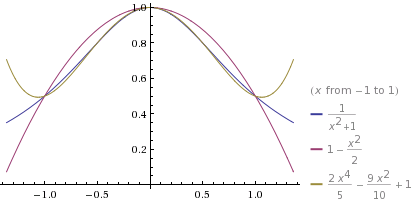
\includegraphics[scale=0.7]{nla_6_1.png}
			\end{figure*} 
 	\end{aufgabe}
	
	\newpage

	\begin{aufgabe}~
		
		Stelle zunächst das Gleichungssystem $Cx+d=r$ auf, setzte dann $A:=C^TC, b:=-C^Td$ und löse $Ax=b$ um die Summe der Fehlerquadrate zu minimieren (Algorithmus aus der Vorlesung).
		\begin{enumerate}
			\item
				Funktionsgleichung: $ax+b$
				\[
					Cx+d:=\begin{pmatrix}0&1\\\f\pi4&1\\\f\pi2&1\\\f{3\pi}4&1\\\pi&1\end{pmatrix}\begin{pmatrix}a\\b\end{pmatrix} + \begin{pmatrix}0\\-\f12\sqrt2\\-1\\-\f12\sqrt{2}\\0\end{pmatrix} = r
				\]
				Löse also
				\[
					Ax:=\begin{pmatrix}\f{57\pi^2}{16} & \f{16\pi}4 \\[0.4em]\f{13\pi}4 & 5\end{pmatrix}\begin{pmatrix}a\\b\end{pmatrix} = \begin{pmatrix}\f\pi2+\f{7\pi}{4\sqrt2}\\[0.4em]1+\sqrt2\end{pmatrix}
				\]
				Es ergibt sich
				\[
					0.03692352x + 0.4074436
				\]
			\item
				Funktionsgleichung: $ax^2+bx+c$
				\[
					Cx+d:=\begin{pmatrix}0&0&1\\[0.3em]\f{\pi^2}{16}&\f{\pi}4&1\\[0.3em]\f{\pi^2}4&\f{\pi}2&1\\[0.3em]\f{9\pi^2}{16}&\f{3\pi}4&1\\[0.3em]\pi^2&\pi&1\end{pmatrix}\begin{pmatrix}a\\b\\c\end{pmatrix}+\begin{pmatrix}0\\[0.3em]-\f12\sqrt2\\[0.3em]-1\\[0.3em]-\f12\sqrt{2}\\[0.3em]0\end{pmatrix} = r
				\]
				Löse also
				\[
					Ax := \begin{pmatrix}\f{177\pi^4}{128} & \f{127\pi^3}{64} & \f{15\pi^2}8\\[0.4em]\f{127\pi^3}{64} & \f{57\pi^2}{16} & \f{13\pi}4\\[0.4em] \f{15\pi^2}8 & \f{13\pi}4 & 5\end{pmatrix}\begin{pmatrix}a\\b\\c\end{pmatrix} = \begin{pmatrix}\f{\pi^2}4+\f{5\pi^2}{8\sqrt{2}}\\[0.4em]\f{\pi}2+\f{7\pi}{4\sqrt{2}}\\[0.4em]1+\sqrt{2}\end{pmatrix}
				\]
				Es ergibt sich
				\[
					-0.1111712x^2 + 0.2213359x + 0.4423227
				\]
		\end{enumerate}
		\begin{note}
			Die Ergebnisse sind wohl nicht ganz richtig.
			Jedenfalls sehen die Graphen dazu nicht sonderlich vernünftig aus.
		\end{note}
	\end{aufgabe}
	\newpage
	\begin{aufgabe}~

		Es gilt
		\begin{align*}
			\begin{vmatrix}
				1 & x_0 & x_0^2 & \cdots & x_0^n\\
				1 & x_1 & x_1^2 & \cdots & x_1^n\\
  \vdots & \vdots & \vdots & \ddots & \vdots \\
				   1 & x_n & x_n^2 & \cdots & x_n^n
			\end{vmatrix}
			&= \begin{vmatrix}
				1 & 0 & 0 & \cdots & 0\\
				1 & x_1-x_0 & x_1^2 - x_0x_1 & \cdots & x_1^n - x_0x_1^{n-1}\\
  \vdots & \vdots & \vdots & \ddots & \vdots\\
				   1 & x_n-x_0 & x_n^2-x_0x_n & \cdots & x_n^n - x_0x_n^{n-1}
			\end{vmatrix}\\
			&= \begin{vmatrix}
				x_1 - x_0 & x_1(x_1-x_0) & x_1^2(x_1-x_0) & \cdots & x_1^{n-1}(x_1-x_0)\\
			 x_2 - x_0 & x_2(x_2-x_0) & x_2^2(x_2-x_0) & \cdots & x_2^{n-1}(x_2-x_0)\\
				   \vdots & \vdots & \vdots & \ddots & \vdots\\
			 x_n - x_0 & x_n(x_n-x_0) & x_n^2(x_n-x_0) & \cdots & x_n^{n-1}(x_n-x_0)
			\end{vmatrix}\\
			&= \prod_{j=1}^n(x_j-x_0) \cdot \begin{vmatrix}
			 1 & x_1 & x_1^2 & \cdots & x_1^{n-1}\\
				1 & x_2 & x_2^2 & \cdots & x_2^{n-1}\\
  \vdots & \vdots & \vdots & \ddots & \vdots \\
				   1 & x_n & x_n^2 & \cdots & x_n^{n-1}
			\end{vmatrix}
			\intertext{Es ergibt sich eine kleinere Matrix, die die gleiche Form, wie die Ursprungsmatrix hat.
			Unter Beachtung der sich verändernden Indizierung ergibt sich somit:}
			&=\prod_{i=0}^{n-1}\left(\prod_{j=i+1}^{n} (x_j-x_i)\right)\\
			&=\prod_{0\le i < j\le n}(x_j - x_i)
		\end{align*}
	\end{aufgabe}
\end{document}
